
\documentclass[11pt]{article}
\usepackage[a4paper, total={6in,9in}]{geometry}
\usepackage[parfill]{parskip}    	
\usepackage{graphicx,caption,fancyhdr,xcolor,pdfpages,setspace}
\usepackage{minted}
\usepackage{xcolor}

\usepackage[hypertexnames=false]{hyperref}

\newcommand{\wrt}[1]{\mathrm{d}#1}


\setlength{\fboxsep}{1em}

\hypersetup{
	colorlinks=true,
	linkcolor=darkgray,
	citecolor=red,
	urlcolor=red
}

\urlstyle{same}
\renewcommand{\footnoterule} % Push footnotes to the bottom of the page
	{\vfill\kern -3pt \hrule width 0.4\columnwidth \kern 2.6pt}

\makeatletter
\title{Digital Design with HDL Lab1}
\let\Title\@title
\author{Y3862181 \& Y3899129}
\let\Author\@author
\date{Autumn Term, 2022}
\let\Date\@date
\makeatother


\fancypagestyle{content}{
    \renewcommand{\headrulewidth}{0.4pt}
    \renewcommand{\footrulewidth}{0.4pt}
    \setlength{\headheight}{15pt}
    
	\fancyhf{}
	\fancyhead[L]{\Author}
	\fancyhead[R]{\Title}
	\fancyfoot[L]{\Date}
	\fancyfoot[R]{\thepage}
}
\onehalfspacing
\begin{document}
\begin{titlepage}
\centering
{\Huge Lab Report 1}

\vspace{3cm}

{\LARGE \textbf{ Digital Design with HDL}}

\vspace{3cm}

{\huge Y3862181 \& Y3899129}

\vspace{2cm}


{\large Autumn Term, 2022}
\vfill

{\itshape University of York}
\end{titlepage}

\tableofcontents
\newpage

\pagestyle{content}
\section{Introduction}

This lab exposes the process of implementing full-adder circuits using VHDL. A 1-bit full-adder is a digital circuit that has three inputs and two outputs. The first two inputs are the bits that will be added together while the third input serves as a carry bit signal. The first output is the sum and the second one is the carry out. Those carry signals are used in order to connect multiple adders together as well as enable computation that exceeds the total input bits of the adder. For example, when adding two 4-bit numbers together, we could expect a 5-bit value (an overflow), hence the need for the carry signals. 

In task A, a 1-bit full-adder will be designed and tested and in task B, the design from the previous task will be used in order to implement and test a 4-bit full-adder.
\newpage

\section{Task A: Implementation of a Simple Design (1-bit Full-Adder)}

\subsection{VHDL Code}
\begin{minted}{vhdl}
library IEEE;
use IEEE.STD_LOGIC_1164.ALL;

-- Combinational logic for a 1-bit full-adder

entity full_adder_1bit is
    Port ( addend0 : in STD_LOGIC;     -- input 0 of the full-adder
           addend1 : in STD_LOGIC;     -- input 1 of the full-adder
           sum     : out STD_LOGIC;    -- output of the full-adder
           
           carry_in : in STD_LOGIC;    -- carry input of the full-adder
           carry_out : out STD_LOGIC); -- carry output of the full-adder
                                       -- both are used to connect to multiple
                                       -- full-adders
end full_adder_1bit;

architecture Behavioral of full_adder_1bit is

signal P,G,Cprop: STD_LOGIC;           -- internal connections

begin
    
    -- implementation of 1bit full-adder
    
    G <= addend0 and addend1; 
    P <= addend0 xor addend1;
    Cprop <= P and carry_in;
    carry_out <= Cprop or G;
    sum <= P xor carry_in;

end Behavioral;
\end{minted}
\newpage

\subsection {1-bit Full-Adder Schematic}

Figure 1 shows the schematic of a 1-bit full-adder that was produced via the VHDL code in section 2.1.


\begin{figure}[ht]
    \centering
    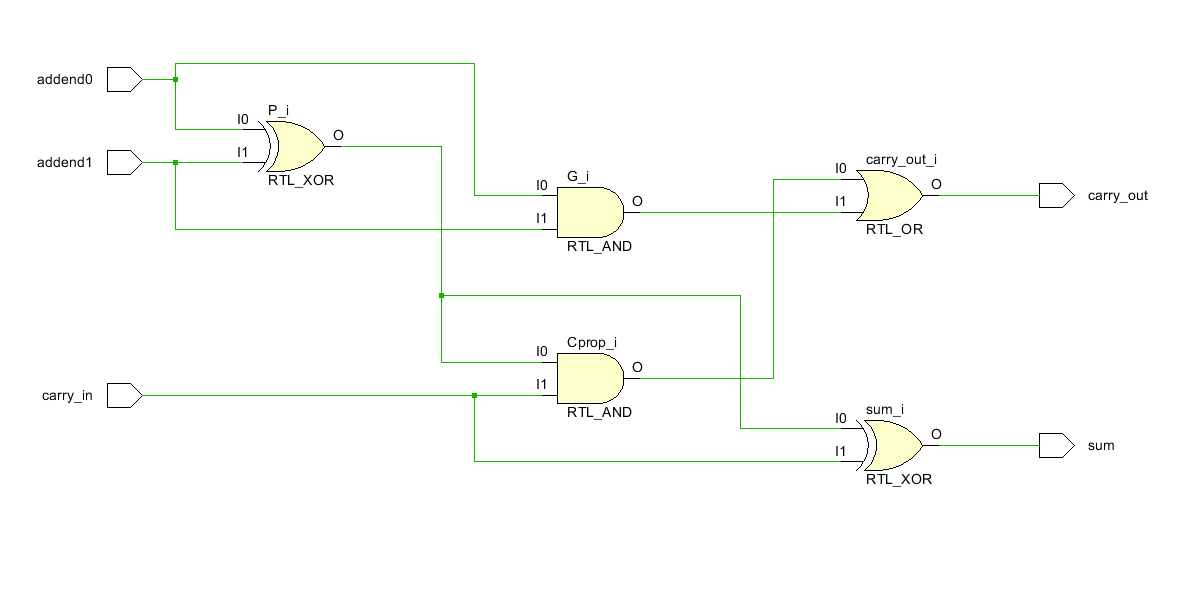
\includegraphics[width=1.0 \textwidth]{schematic_diagram.png}
    \caption{Schematic of a 1bit Full-Adder}
    \label{fig:isa}
\end{figure}

\subsection {RTL Component Statistics for a 1-bit Full-Adder }

Figure 2 is taken from the synthesis report, which illustrates the number of special components used by the implementation of the 1-bit full-adder. This can be used to verify that the design was synthesised correctly for the FPGA device.



\begin{figure}[ht]
    \centering
    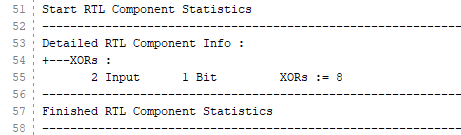
\includegraphics[width=0.8 \textwidth]{RTL_component_statistics.png}
    \caption{RTL component statistics for a 1bit Full-Adder}
    \label{fig:isa}
\end{figure}



\newpage
\subsection{Testbench}

The VHDL code below exposes the process of testing the design of the 1-bit full-adder in a simulation environment:


\begin{minted}{vhdl}
library IEEE;
use IEEE.STD_LOGIC_1164.ALL;

-- Simulation for testing the 1-bit full-adder

entity full_adder_1bit_tb is

end full_adder_1bit_tb;

architecture Behavioral of full_adder_1bit_tb is

signal addend0, addend1 : STD_LOGIC; -- The two inputs of the full-adder
signal carry_in         : STD_LOGIC; -- Carry input of the full-adder
signal sum              : STD_LOGIC; -- Output of the full-adder
signal carry_out        : STD_LOGIC; -- Carry output of the full-adder

begin

UUT: entity work.full_adder_1bit
 PORT MAP (
   addend0   => addend0,
   addend1   => addend1,
   carry_in  => carry_in,
   sum       => sum,
   carry_out => carry_out);

TEST : process
begin
    -- In order to test the full functionality of the full-adder,
    -- we need to simulate all of the possible input signal combinations
    --( addend0, addend1 and carry_in from 0b000 (0) to 0b111 (7) )
    wait for 100 ns;
\end{minted}
\newpage
\begin{minted}{vhdl}
    -- 0b000 (0)
    addend0  <= '0';
    addend1  <= '0';
    carry_in <= '0';
    wait for 10 ns;
    
    -- 0b001 (1)
    addend0  <= '0';
    addend1  <= '0';
    carry_in <= '1';
    wait for 10 ns;
    
    -- 0b010 (2)
    addend0  <= '0';
    addend1  <= '1';
    carry_in <= '0';
    wait for 10 ns;
    
    -- 0b011 (3)
    addend0  <= '0';
    addend1  <= '1';
    carry_in <= '1';
    wait for 10 ns;
    
    -- 0b100 (4)
    addend0  <= '1';
    addend1  <= '0';
    carry_in <= '0';
    wait for 10 ns;
    
    -- 0b101 (5)
    addend0  <= '1';
    addend1  <= '0';
    carry_in <= '1';
    wait for 10 ns;
\end{minted}
\newpage
\begin{minted}{vhdl}
    
    -- 0b110 (6)
    addend0  <= '1';
    addend1  <= '1';
    carry_in <= '0';
    wait for 10 ns;
    
    --- 0b111 (7)
    addend0  <= '1';
    addend1  <= '1';
    carry_in <= '1';
    wait for 10 ns;
    
    wait;
end process;

end Behavioral;
\end{minted}

\subsection{Timing Diagram of a 1-bit Full-Adder}
The timing diagram shown in Figure 3 is produced via the Vivado simulation environment, given the VHDL files for the 1-bit full-adder and the testbench. This timing diagram proves that the 1-bit full-adder designed in Task A is operating as expected. 

It can be observed, for instance, that when the two addend inputs are in a logic high state, the output sum is at a logic low and the carry output signal is at a logic high.

In addition, when all of the inputs are at a logic high, then all of the outputs are at a logic high as well.


\begin{figure}[ht]
    \centering
    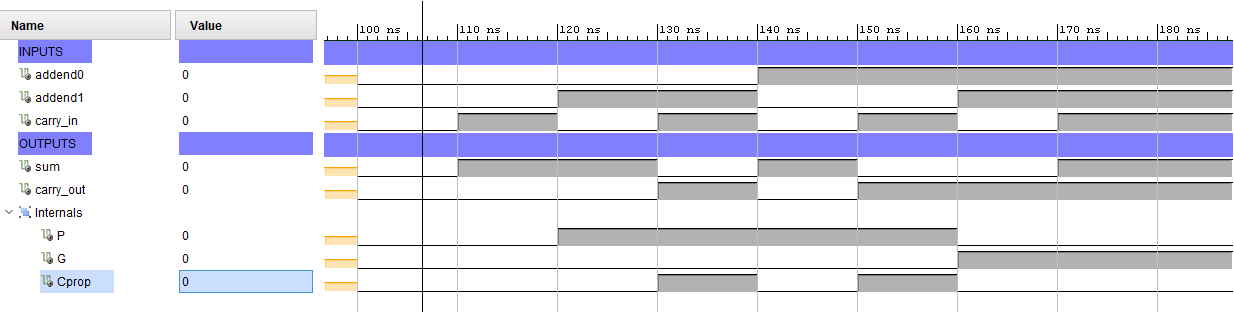
\includegraphics[width=1.0 \textwidth]{timing_diagram.png}
    \caption{Timing diagram of a 1-bit Full-Adder}
    \label{fig:isa}
\end{figure}

\newpage

\subsection{Signal to Pin Assignments for the FPGA}

The signal to pin assignments exposed below are used when uploading the design onto the Zedboard Zynq Evaluation and Development Kit (part number xc7z020clg484-1):

\hspace{10mm}
\begin{minted}{text}
# Signals to pin assignments

# carry_in -> F22
set_property PACKAGE_PIN F22 [get_ports {carry_in}]
set_property IOSTANDARD LVCMOS18 [get_ports {carry_in}]

# addend0 -> G22
set_property PACKAGE_PIN G22 [get_ports {addend0}]
set_property IOSTANDARD LVCMOS18 [get_ports {addend0}]

# addend1 -> H22
set_property PACKAGE_PIN H22 [get_ports {addend1}]
set_property IOSTANDARD LVCMOS18 [get_ports {addend1}]

# sum -> T22
set_property PACKAGE_PIN T22 [get_ports {sum}]
set_property IOSTANDARD LVCMOS18 [get_ports {sum}]

# carry_out -> T21
set_property PACKAGE_PIN T21 [get_ports {carry_out}]
set_property IOSTANDARD LVCMOS18 [get_ports {carry_out}]
\end{minted}


\newpage
\section{Task B: Implementation of Components }

\subsection{VHDL Code}

\begin{minted}{vhdl}
library IEEE;
use IEEE.STD_LOGIC_1164.ALL;

-- Implementation of a 4-bit full-adder relying on the previous implementation
-- of a 1-bit full-adder

entity full_adder_4bit is
    Port ( first_addend  : in STD_LOGIC_VECTOR (3 downto 0);     -- first input bus
           second_addend : in STD_LOGIC_VECTOR (3 downto 0);     -- second input bus
           carry_in      : in STD_LOGIC;                         -- input carry 
           sum           : out STD_LOGIC_VECTOR (3 downto 0);    -- output bus
           carry_out     : out STD_LOGIC );                      -- output carry
end full_adder_4bit;

architecture Behavioral of full_adder_4bit is

-- Internal inputs which connect the carries between the discrete 1-bit full-adders
-- carry_fa_[carry out index | carry in index]

signal carry_fa_01: STD_LOGIC;
signal carry_fa_12: STD_LOGIC;
signal carry_fa_23: STD_LOGIC;

begin

-- Index 0 full-adder
fa_0 : entity work.full_adder_1bit
port map (
    addend0  => first_addend(0),
    addend1  => second_addend(0),
    carry_in => carry_in,
    sum => sum(0),
    carry_out => carry_fa_01
);
\end{minted}
\newpage
\begin{minted}{vhdl}
-- Index 1 full-adder
fa_1 : entity work.full_adder_1bit
port map (
    addend0  => first_addend(1),
    addend1  => second_addend(1),
    carry_in => carry_fa_01,
    sum => sum(1),
    carry_out => carry_fa_12
);

-- Index 2 full-adder
fa_2 : entity work.full_adder_1bit
port map (
    addend0  => first_addend(2),
    addend1  => second_addend(2),
    carry_in => carry_fa_12,
    sum => sum(2),
    carry_out => carry_fa_23
);

-- Index 3 full-adder
fa_3 : entity work.full_adder_1bit
port map (
    addend0  => first_addend(3),
    addend1  => second_addend(3),
    carry_in => carry_fa_23,
    sum => sum(3),
    carry_out => carry_out
);

end Behavioral;
\end{minted}
\newpage
\subsection{4-bit Full-Adder Schematic}
Figure 4 shows the schematic of a 4-bit full-adder that was produced via the VHDL code in section 3.1:
\begin{figure}[ht]
    \centering
    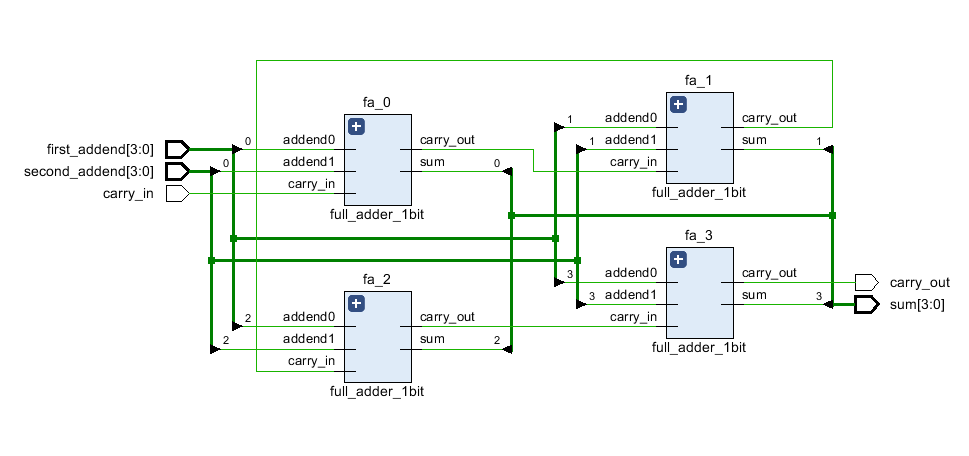
\includegraphics[width=1.0 \textwidth]{rtl_schematic.png}
    \caption{RTL Schematic of a 4bit Full-Adder}
    \label{fig:isa}
\end{figure}

\subsection {RTL Component Statistics for a 4-bit Full-Adder }

Figure 5 is taken from the synthesis report, which illustrates the number of special components used by the implementation of the 4-bit full-adder. This can be used to verify that the design was synthesised correctly for the FPGA device.



\hspace{5mm}

\begin{figure}[ht]
    \centering
    \includegraphics[width=0.7 \textwidth]{rtl_component_statistics.png}
    \caption{RTL Component Statistics for a 4-bit Full-Adder}
    \label{fig:isa}
\end{figure}
\newpage


\subsection {Testbench}
The VHDL code below exposes the process of testing the design of the 4-bit full-adder in a simulation environment. Since there are $2^9$ combinations, it would be inefficient to test all of them. Thus, a testing strategy was implemented and described below:

\begin{minted}{vhdl}
library IEEE;
use IEEE.STD_LOGIC_1164.ALL;

-- Testbench for a 4-bit full-adder

entity full_adder_4bit_tb is

end full_adder_4bit_tb;

architecture Behavioral of full_adder_4bit_tb is

signal first_addend  : STD_LOGIC_VECTOR (3 downto 0);   -- first input bus
signal second_addend : STD_LOGIC_VECTOR (3 downto 0);   -- second input bus
signal carry_in      : STD_LOGIC;                       -- input carry
signal sum           : STD_LOGIC_VECTOR (3 downto 0);   -- output bus
signal carry_out     : STD_LOGIC;                       -- output carry

begin 

UUT: entity work.full_adder_4bit
    PORT MAP (
        first_addend  => first_addend,
        second_addend => second_addend,
        carry_in => carry_in,
        sum => sum,
        carry_out => carry_out
    );

-- TESTING STRATEGY: This TB verifies the design of a 4bit full-adder.
-- The adder uses trusted 1bit full-adders as components in a 
-- ripple-carry configuration.
-- The test patters have been selected to verify that the 1bit 
-- adders have been connected correctly. This is done by first testing
-- the cleared state. Then testing if all of the separate carry signals
-- work, including the overflow state. And finally, test the case
-- of mixed value summation

TEST : process
begin

    wait for 100 ns;
    
    -- testing clear state
    first_addend  <= "0000";
    second_addend <= "0000";
    carry_in <= '0';
    wait for 10 ns;
    
    -- testing the external carry in
    first_addend  <= "0000";
    second_addend <= "0000";
    carry_in <= '0';
    wait for 10 ns;
    
    -- testing first internal carry
    first_addend  <= "0001";
    second_addend <= "0001";
    carry_in <= '0';
    wait for 10 ns;
    
    -- testing second internal carry
    first_addend  <= "0010";
    second_addend <= "0010";
    carry_in <= '0';
    wait for 10 ns;
    
     -- testing third internal carry
    first_addend  <= "0100";
    second_addend <= "0100";
    carry_in <= '0';
    wait for 10 ns;
\end{minted}
\newpage
\begin{minted}{vhdl}
    -- testing external carry out
    first_addend  <= "1000";
    second_addend <= "1000";
    carry_in <= '0';
    wait for 10 ns;
    
    -- testing the overflow state
    first_addend  <= "1111";
    second_addend <= "1111";
    carry_in <= '1';
    wait for 10 ns;
    
    -- testing mixed state value
    first_addend  <= "1110";
    second_addend <= "0011";
    carry_in <= '0';
    wait for 10 ns;
    
    wait;
end process;

end Behavioral;
\end{minted}


\subsection{Timing Diagram of a 4-bit Full-Adder}
The timing diagram shown in Figure 6 is produced via the Vivado simulation environment, given the VHDL files for the 4-bit full-adder and the testbench. This timing diagram proves that the 4-bit full-adder designed in Task B is operating as expected.
\hspace{20mm}

\begin{figure}[ht]
    \centering
    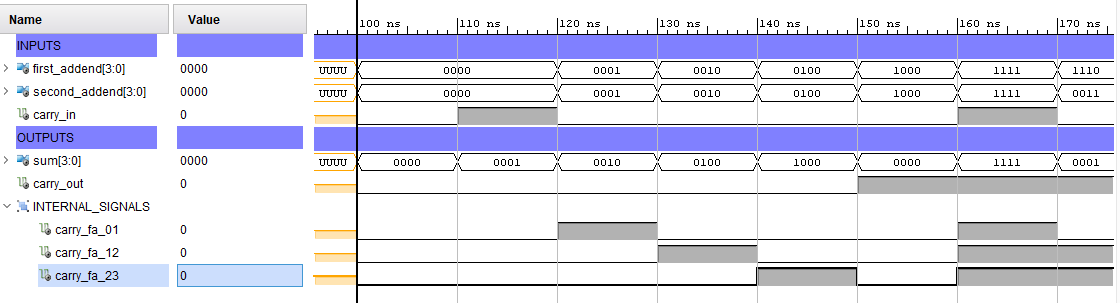
\includegraphics[width=1.0 \textwidth]{simulation.png}
    \caption{Timing diagram of a 4-bit Full-Adder}
    \label{fig:isa}
\end{figure}


\section {Conclusion}

Both a 1-bit and 4-bit full-adder circuits were successfully implemented in VHDL. The testbenches have confirmed that the implementations are operating correctly. 

In addition, the 1-bit full-adder was compiled and uploaded onto the Zedboard, hence it was tested manually using switches for the inputs and diodes for the outputs.

\end{document}  